%\hypertarget{___gatsby}{}
%\hypertarget{gatsby-focus-wrapper}{}
%\href{https://mukulrathi.com/}{}
%
%MUKUL RATHI
%
%\href{https://mukulrathi.com/about-me}{}
%
%About Me
%
%\href{https://mukulrathi.com/blog}{}
%
%Blog
%
%\hypertarget{creating-the-bolt-compiler-part-5}{%
%\subsection{Creating the Bolt Compiler: Part
%5}\label{creating-the-bolt-compiler-part-5}}

\hypertarget{top-of-page}{%
\chapter{A tutorial on liveness and alias dataflow
analysis}\label{top-of-page}}

June 27, 2020

%\hypertarget{june-27-2020}{%
%\subsection{June 27, 2020}\label{june-27-2020}}
%
%\hypertarget{min-read}{%
%\subsection{7 min read}\label{min-read}}
%
%\hypertarget{last-updated-december-20-2020}{%
%\subsection{Last updated: December 20,
%2020}\label{last-updated-december-20-2020}}
%
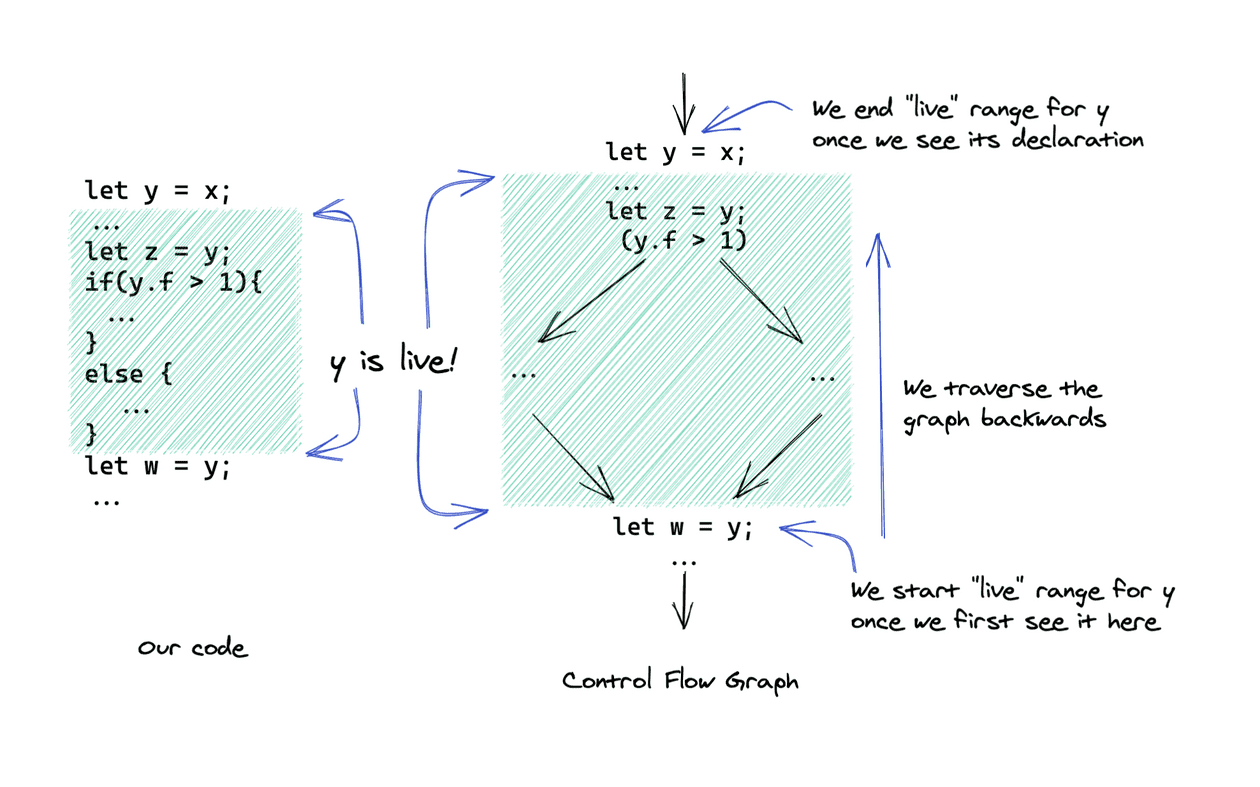
\includegraphics[width=\linewidth]{05_files/liveness-range.png}
%
%\hypertarget{series-creating-the-bolt-compiler}{%
%\section{Series: Creating the Bolt
%Compiler}\label{series-creating-the-bolt-compiler}}
%
%\begin{itemize}
%\item
%  { Part 1:
%  }\href{https://mukulrathi.com/create-your-own-programming-language/intro-to-compiler/}{How
%  I wrote my own "proper" programming language}
%\item
%  { Part 2:
%  }\href{https://mukulrathi.com/create-your-own-programming-language/compiler-engineering-structure/}{So
%  how do you structure a compiler project?}
%\item
%  { Part 3:
%  }\href{https://mukulrathi.com/create-your-own-programming-language/parsing-ocamllex-menhir/}{Writing
%  a Lexer and Parser using OCamllex and Menhir}
%\item
%  { Part 4:
%  }\href{https://mukulrathi.com/create-your-own-programming-language/intro-to-type-checking/}{An
%  accessible introduction to type theory and implementing a
%  type-checker}
%\item
%  \textbf{Part 5: A tutorial on liveness and alias dataflow analysis}
%\item
%  { Part 6:
%  }\href{https://mukulrathi.com/create-your-own-programming-language/lower-language-constructs-to-llvm/}{Desugaring
%  - taking our high-level language and simplifying it!}
%\item
%  { Part 7:
%  }\href{https://mukulrathi.com/create-your-own-programming-language/protobuf-ocaml-cpp-tutorial/}{A
%  Protobuf tutorial for OCaml and C++}
%\item
%  { Part 8:
%  }\href{https://mukulrathi.com/create-your-own-programming-language/llvm-ir-cpp-api-tutorial/}{A
%  Complete Guide to LLVM for Programming Language Creators}
%\item
%  { Part 9:
%  }\href{https://mukulrathi.com/create-your-own-programming-language/concurrency-runtime-language-tutorial/}{Implementing
%  Concurrency and our Runtime Library}
%\item
%  { Part 10:
%  }\href{https://mukulrathi.com/create-your-own-programming-language/generics-parametric-polymorphism/}{Generics
%  - adding polymorphism to Bolt}
%\item
%  { Part 11:
%  }\href{https://mukulrathi.com/create-your-own-programming-language/inheritance-method-overriding-vtable/}{Adding
%  Inheritance and Method Overriding to Our Language}
%\end{itemize}
%
%\begin{center}\rule{0.5\linewidth}{0.5pt}\end{center}

\hypertarget{dataflow-analysis---the-big-picture}{%
\section{\texorpdfstring{\protect\hyperlink{dataflow-analysis---the-big-picture}{}Dataflow
Analysis - the big
picture}{Dataflow Analysis - the big picture}}\label{dataflow-analysis---the-big-picture}}

In the previous post in the series, we looked at how type-checking the
core language worked. This analysis is \emph{flow-insensitive} - it does
not depend on the flow of the execution of the program. If an expression
is of type \texttt{int} then it will have type \texttt{int} regardless
of what was executed before or after it.

Some program properties do however depend on the execution path taken by
a program. Dataflow analysis tracks how a particular value might
propagate as the program executes.

For example, a value might \emph{alias} - you could have multiple
references pointing to that value. Whether two references \texttt{x} and
\texttt{y} alias can't be determined by looking at their assignments in
isolation - we need to track the execution to determine if they have the
same value assigned to them.

%{alias\_example}

%Copy

\begin{verbatim}
let x = someObject...
let y = someObject 
// x and y alias as both point to same object
\end{verbatim}

Another example is \textbf{liveness analysis} - we say a value is
\emph{live} if some point later in the program it could be used, and
\emph{dead} otherwise.

%{liveness\_example}

%Copy

\begin{verbatim}
let x = someValue 
// someValue is live...
print(x) // as we use someValue here
x = someOtherValue 
// someOtherValue isn't used - so dead
\end{verbatim}

Why do we care about alias analysis and liveness analysis? Well it turns
out that Rust's \emph{borrow-checker} uses a combination of these to
determine when a reference is borrowed. Bolt has a \emph{linear}
capability in its type system which acts the same.

Both Rust's borrow checker and Bolt's capabilities prevent data races -
an explanation why is in
\href{https://github.com/mukul-rathi/bolt-dissertation/blob/master/dissertation.pdf}{my
dissertation}.

In a nutshell, Rust works on the principle of \textbf{ownership}: you
either have one reference (owner) that can read/write (a \emph{mutable}
reference) or you can \emph{borrow} (aka alias) the reference.

To enforce this we care about 2 things:

\begin{enumerate}
\tightlist
\item
  When is a reference borrowed? (alias analysis)
\item
  For how long is it borrowed? (liveness analysis)
\end{enumerate}

Let's elaborate on that second point. When is a reference borrowed? The
first version of Rust's borrow checker said this was whilst an alias was
in scope.

{borrow\_example}

Copy

\begin{verbatim}
let x = something 
// this is pseudocode not Rust
{  let y = x  ...
   // y will be used in future
  print(y)
  // no longer using y
  x = somethingElse
}// y is out of scope
\end{verbatim}

That means we cannot reassign \texttt{x} in the example until \texttt{y}
is out of scope. This is a ``lexical lifetime'' - \texttt{y}'s borrow
lifetime is determined by its lexical scope. So that means \texttt{x}
can't be reassigned, since it is borrowed at that point. But \texttt{y}
isn't being used so surely \texttt{x} isn't still borrowed?

That's the idea behind \textbf{non-lexical lifetimes} - the borrow ends
when the value of \texttt{y} is dead - i.e. it is not being used.

In Bolt, we'll be tracking the lifetimes of references to
\emph{objects}.

Let's get implementing it!

\hypertarget{alias-analysis}{%
\section{\texorpdfstring{\protect\hyperlink{alias-analysis}{}Alias
Analysis}{Alias Analysis}}\label{alias-analysis}}

The first step is to determine when two values alias. How do we know two
references will point to the same object without actually executing the
program?

We use \textbf{abstract interpretation}.

\hypertarget{abstract-interpretation}{%
\subsection{\texorpdfstring{\protect\hyperlink{abstract-interpretation}{}Abstract
Interpretation}{Abstract Interpretation}}\label{abstract-interpretation}}

Abstract interpretation is the process of simulating the execution of
the program but only storing the program properties we care about. So in
our case, we don't care about what the actual result of the program
execution is, we're just tracking the \emph{set of aliases}.

Implicit in this is a set of rules for how the program will execute, we
call this its \textbf{operational semantics}. We will not go into
details here, but it's things like:

\begin{itemize}
\tightlist
\item
  Do we evaluate expressions left-to-right or right-to-left?
\item
  When calling a function, do we fully evaluate the argument expression
  and then call the function with the value of that argument, or do we
  just plug in the unevaluated argument expression directly into the
  function and only evaluate it at the point it is used in the function
  body? The former is called \textbf{call-by-value} and is used in most
  mainstream languages like Java and Python, the latter is called
  \textbf{call-by-name} and is used in Haskell and Lisp.
\end{itemize}

There's a lot more to say about this - perhaps it's worthy of its own
blog post? Send me a tweet if you would like one!

When do we have aliasing? When a new variable is declared or when it is
reassigned. For simplicity (and also because we don't want the lifetime
of the alias to be larger than the original value) we will not allow
aliasing via reassigning an existing variable (e.g. \texttt{x\ :=\ y}).

So we care about expressions of this form:

Copy

\begin{verbatim}
let x = e
\end{verbatim}

The expression \texttt{e} can \emph{reduce} to a value when executing
e.g. \texttt{1+2} reduces to \texttt{3}. If when executing \texttt{e} it reduces to a reference \texttt{y}, then
the overall expression would look like:

%Copy

\begin{verbatim}
let x = y
\end{verbatim}

And so \texttt{x} would alias \texttt{y}. So let's write a function
that, given an expression, will return the list of identifiers that it
could possible reduce to. That'll tell us what \texttt{x} could possibly
alias.

We'll store this helper function in an ``environment'' of helper
functions used in the data-race type-checking stage of the Bolt
compiler: \texttt{data\_race\_checker\_env.mli}

The type signature of this OCaml function is as we'd expect:

%{
%\href{https://github.com/mukul-rathi/bolt/blob/master/src/frontend/data_race_checker/data_race_checker_env.mli}{data\_race\_checker\_env.mli}}
%
%Copy

\begin{lstlisting}[language=caml,caption={data\_race\_checker\_env.mli}]
val reduce_expr_to_obj_ids : expr -> identifier list
\end{lstlisting}

A reminder of the type of \texttt{expr} defined in the
\href{https://mukulrathi.com/create-your-own-programming-language/intro-to-type-checking/\#annotating-our-ast-with-types}{previous
post} - \texttt{loc} encodes the line number and position of the
expression - used for error messages.

%{
%\href{https://github.com/mukul-rathi/bolt/blob/simple-compiler-tutorial/src/frontend/typing/typed_ast.mli}{typed\_ast.mli}}
%
%Copy

\begin{lstlisting}[language=caml,caption={typed\_ast.mli}]
type identifier =
  | Variable of type_expr * Var_name.t
  | ObjField of Class_name.t * Var_name.t * type_expr * Field_name.t
      (** class of the object, type of field *)
type expr =
  | Integer     of loc * int
  | Boolean     of loc * bool
  | Identifier  of loc * identifier
  | Constructor of loc * type_expr * Class_name.t * constructor_arg list
  | Let         of loc * type_expr * Var_name.t * expr
  | Assign      of loc * type_expr * identifier * expr
  | If          of loc * type_expr * expr * block_expr * block_expr
  ...

and block_expr =
  | Block of loc * type_expr * expr list
\end{lstlisting}

%\begin{verbatim}
%type identifier =  | Variable of type_expr * Var_name.t  | ObjField of Class_name.t * Var_name.t * type_expr * Field_name.t      (** class of the object, type of field *)type expr =  | Integer     of loc * int  | Boolean     of loc * bool  | Identifier  of loc * identifier  | Constructor of loc * type_expr * Class_name.t * constructor_arg list  | Let         of loc * type_expr * Var_name.t * expr  | Assign      of loc * type_expr * identifier * expr  | If          of loc * type_expr * expr * block_expr * block_expr  ...
%and block_expr =  | Block of loc * type_expr * expr list
%\end{verbatim}

Starting off with the simple cases, it's clear an integer or a boolean
value doesn't reduce to an identifier, and an identifier expression
reduces to that identifier. A \texttt{new\ SomeClass()} constructor also
doesn't reduce to an identifier.

%{
%\href{https://github.com/mukul-rathi/bolt/blob/master/src/frontend/data_race_checker/data_race_checker_env.ml}{data\_race\_checker\_env.ml}}
%
%Copy

\begin{lstlisting}[language=caml,caption={data\_race\_checker\_env.ml}]
let rec reduce_expr_to_obj_ids expr =
  match expr with
  | Integer _ | Boolean _ -> []
  | Identifier (_, id) -> [id]
  | Constructor (_, _, _, _) -> []
\end{lstlisting}

If we have a let expression or assigning to an identifier, then it
reduces to that identifier (e.g. \texttt{let\ x\ =\ \_\_\_} reduces to
\texttt{x}, and \texttt{x.f:=\ \_\_} reduces to \texttt{x.f}):

%{
%\href{https://github.com/mukul-rathi/bolt/blob/master/src/frontend/data_race_checker/data_race_checker_env.ml}{data\_race\_checker\_env.ml}}
%
%Copy

\begin{lstlisting}[language=caml]
...  
  | Let (_, _, _, bound_expr) -> reduce_expr_to_obj_ids bound_expr
  | Assign (_, _, _, assigned_expr) -> reduce_expr_to_obj_ids assigned_expr
\end{lstlisting}

We can continue doing this for other cases. But what about an
\texttt{if} statement? Does this expression reduce to \texttt{x} or
\texttt{y}?

%Copy

\begin{verbatim}
if (someCondition) {  x} else {  y}
\end{verbatim}

In general, without actually executing the expression, we don't know. So
we'll have to approximate.

Let's remind ourselves of our goal - to mark a value as borrowed/not
linear (Rust / Bolt equiv. terminology) if it is aliased. We're trying
to eliminate data races, so we have to be \emph{conservative} - assume
it might be aliased even if it isn't. The worst thing would be to let a
data race slip through. Abstract interpretation \emph{always} errs on
the side of soundness.

So we'll \emph{overapproximate} the list of possible identifiers the
expression could reduce to - we don't know which branch so we'll count
the identifiers from \emph{both} branches.

%{
%\href{https://github.com/mukul-rathi/bolt/blob/master/src/frontend/data_race_checker/data_race_checker_env.ml}{data\_race\_checker\_env.ml}}
%
%Copy

\begin{lstlisting}[language=caml]
...
  | If (_, _, _, then_expr, else_expr) ->
      let then_ids = reduce_block_expr_to_obj_ids then_expr in
      let else_ids = reduce_block_expr_to_obj_ids else_expr in
      then_ids @ else_ids
\end{lstlisting}

So in the example above, we'd return a list \texttt{{[}x,\ y{]}}.

\hypertarget{computing-all-aliases}{%
\subsection{\texorpdfstring{\protect\hyperlink{computing-all-aliases}{}Computing
all aliases}{Computing all aliases}}\label{computing-all-aliases}}

So we know if we have an expression \texttt{let\ y\ =\ e} and \texttt{e}
reduces to \texttt{x}, then we have \texttt{let\ y\ =\ x} and so
\texttt{y} is an alias of \texttt{x}.

In the expression below, we would also run abstract interpretation
(simple in this case) to find that \texttt{z} and \texttt{w} are aliases
of \texttt{y}.

%Copy

\begin{verbatim}
let y = x...
let z = y
if(y.f > 1){  ...}
else {
}
...
let w = y
\end{verbatim}

By transitivity, \texttt{z} and \texttt{w} must also be aliases of
\texttt{x}.

I like to think of this like a graph where each edge is a
direct/immediate alias. We can find all aliases, by repeatedly applying
abstract interpretation in a ``breadth-first search'' style - each
iteration we're expanding the frontier. And each iteration we try to
find aliases of the aliases we've found - so the first iteration we find
aliases of \texttt{x}, then the next iteration we find aliases of
\texttt{x} and \texttt{y} and so on\ldots{}

{
\href{https://mukulrathi.com/static/e996478c0eaa723fc8028caa72847284/191e2/alias-frontier.png}{{}
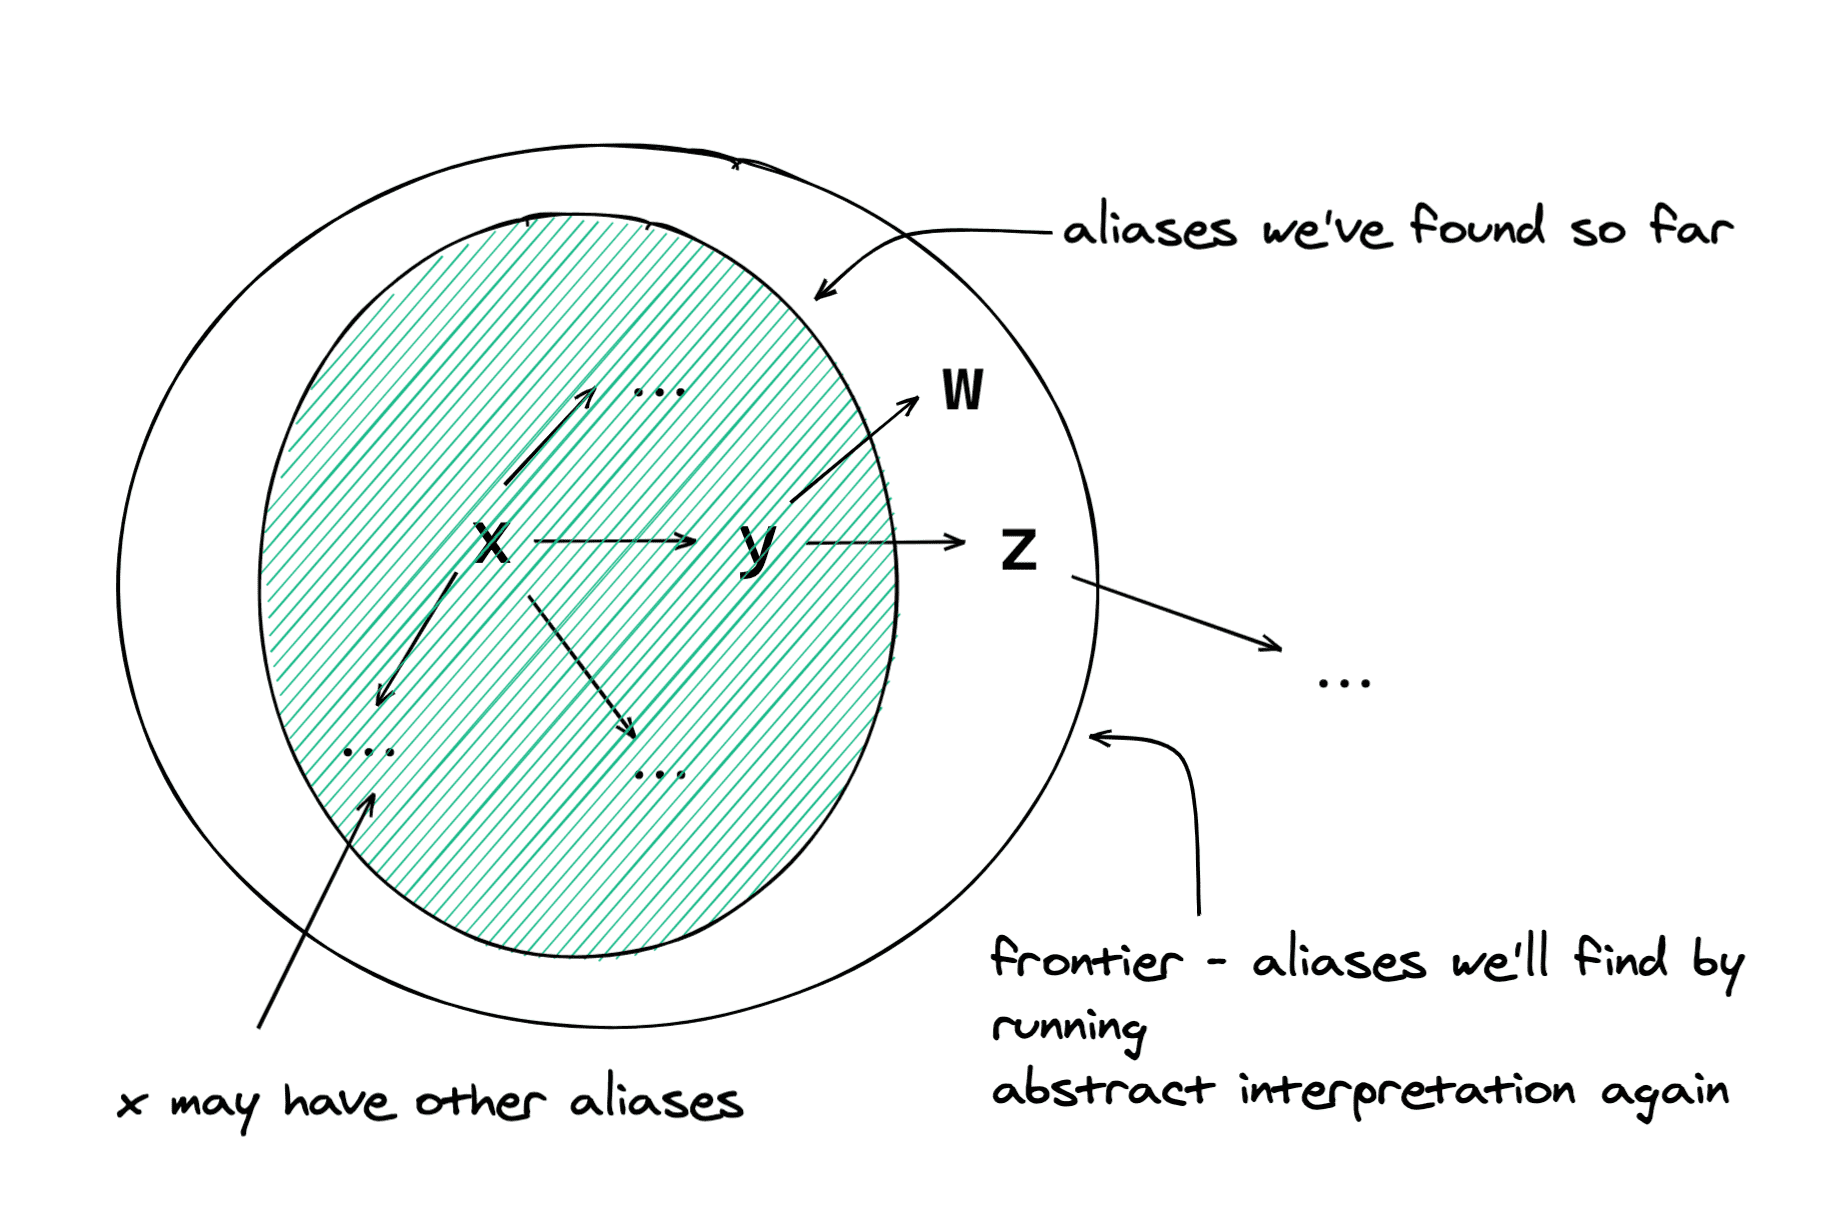
\includegraphics[width=\linewidth]{05_files/alias-frontier.png}} }

So we repeat, until we find no more aliases. The full code is linked in
the repo, and includes an option of matching fields (i.e. should we
consider aliases of \texttt{x.f} as well as \texttt{x}?) We won't in
this case, but other aspects of Bolt's data-race type-checker do use
this.

But the beauty of functional programming is that the function says what
we're doing with no boilerplate:

%{
%\href{https://github.com/mukul-rathi/bolt/blob/master/src/frontend/data_race_checker/data_race_checker_env.ml}{data\_race\_checker\_env.ml}}
%
%Copy

\begin{lstlisting}[language=caml]
let rec get_all_obj_aliases should_match_fields curr_aliases block_expr =
    find_immediate_aliases_in_block_expr should_match_fields name_to_match curr_aliases
      block_expr
    |> fun updated_aliases ->
    if var_lists_are_equal updated_aliases curr_aliases
       then curr_aliases (* we're done! *)
    else get_all_obj_aliases should_match_fields updated_aliases block_expr
    (* repeat with an expanded frontier *)
\end{lstlisting}

\hypertarget{liveness-analysis}{%
\section{\texorpdfstring{\protect\hyperlink{liveness-analysis}{}Liveness
Analysis}{Liveness Analysis}}\label{liveness-analysis}}

Alright, so we're halfway there - we've identified our aliases, now we
need to find out when they're live. Remember a value is \emph{live} if
there's some program execution path in the future it will be used on.

\hypertarget{control-flow-graph}{%
\subsection{\texorpdfstring{\protect\hyperlink{control-flow-graph}{}Control
Flow Graph}{Control Flow Graph}}\label{control-flow-graph}}

To do this, let's formalise the notion of ``execution paths'' in a
program. We're going to be representing a program as a graph of
instructions, with edges representing the steps in the execution. We
call this the \textbf{Control Flow Graph} of the program.

However, if every statement represented a node on the graph, with edges
between them, the graph would be incredibly large (a 100 line program
would have 100 statements). We can be a bit cleverer and group together
statements that will always execute right after each other.

If there's only \textbf{one path} from the start statement to the end
statement in a group of statements, we can represent this as a
\textbf{single node} in our control flow graph. We call this node a
\textbf{basic block} of statements. Below you can see the lines of code
highlighted in different colours to show which basic block they lie in.

\begin{figure}
\centering
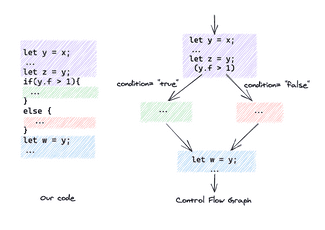
\includegraphics[width=\linewidth]{05_files/control-flow-graph.png}
\caption{Note how the control flow graph shows two different execution
paths, corresponding to the if-else branch taken.}
\end{figure}

In our graph, we can pick any statement in the program and ask, is the
value of variable \texttt{y} live at this point?

A naive way of checking this is to traverse the graph forwards until you
see a use of this value of \texttt{y} (so \texttt{y} is live) or until
you reach the end (you therefore know \texttt{y} is dead). But this is
hopelessly wasteful - for every statement we have to go forward and
traverse the graph to check if the variable's are used.

We can look at it another way, if we traverse \emph{backwards}, then the
first use of \texttt{y} that we encounter is the last use if we
traversed it going forwards. So as soon as we see \texttt{y} being used
when we go backwards, we know that whilst \texttt{y} is defined, it is
live.

A picture helps so let's look at our graph:

{
\href{https://mukulrathi.com/static/12ada8741740841a048f22702b12b7f9/5b503/liveness-range.png}{{}
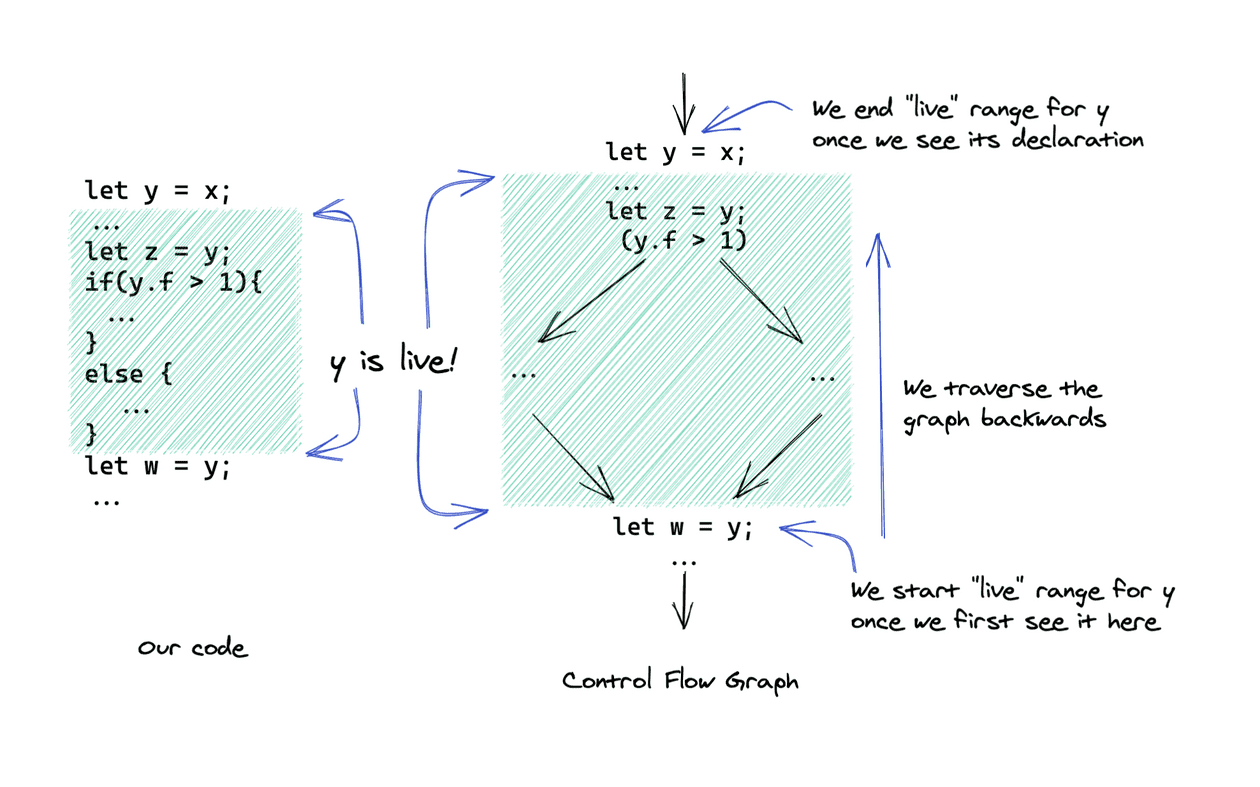
\includegraphics[width=\linewidth]{05_files/liveness-range.png}} }

So to summarise, in liveness analysis we:

\begin{itemize}
\tightlist
\item
  Traverse the Control Flow Graph backwards
\item
  Keep track of the set of live values
\item
  If we see a value for the first time, we add it to our set
\item
  We remove a value if we see its definition
\end{itemize}

\hypertarget{implementing-our-alias-liveness-checker}{%
\section{\texorpdfstring{\protect\hyperlink{implementing-our-alias-liveness-checker}{}Implementing
Our Alias Liveness
Checker}{Implementing Our Alias Liveness Checker}}\label{implementing-our-alias-liveness-checker}}

Now we have our theoretical understanding in place, let's implement the
checker.
%
Whenever we encounter an identifier, we need to know what the original
object reference was, the set of possible aliases, and separately those
that are live.

%{
%\href{https://github.com/mukul-rathi/bolt/blob/master/src/frontend/data_race_checker/type_alias_liveness.ml}{type\_alias\_liveness.ml}}
%
%Copy

\begin{lstlisting}[caption={type\_alias\_liveness.ml},language=caml]
let type_alias_liveness_identifier obj_name possible_aliases
  filter_linear_caps_fn live_aliases id =
  let id_name = get_identifier_name id in
\end{lstlisting}

Our function deals with three cases depending on the identifier name:

\begin{itemize}
\tightlist
\item
  It is the original object reference
\item
  It is a possible alias
\item
  It is another reference we don't care about
\end{itemize}

In the first case, we want to filter the linear capabilities (since the
reference is not linear so can't use them) if there are live aliases.
Along with the updated identifier, we also return the unchanged set of
live aliases.

\begin{lstlisting}[caption={type\_alias\_liveness.ml},language=caml]
if id_name = obj_name then (* original object reference *)
    let maybe_updated_capabilities =
      update_capabilities_if_live_aliases filter_linear_caps_fn
      live_aliases (get_identifier_capabilities id) in
    (set_identifier_capabilities id maybe_updated_capabilities, live_aliases)
\end{lstlisting}


Otherwise, we need to check if the identifier is one of the possible
aliases - if so we add it to the set of live aliases we are tracking. So
we then return this updated set of live aliases along with the
identifier.

%{
%\href{https://github.com/mukul-rathi/bolt/blob/master/src/frontend/data_race_checker/type_alias_liveness.ml}{type\_alias\_liveness.ml}}
%
%Copy


\begin{lstlisting}[language=caml]
else
  ( match
      List.find
        ~f:(fun poss_alias ->
                identifier_matches_var_name poss_alias id)
        possible_aliases
    with
  | Some alias -> alias :: live_aliases
  | None       -> live_aliases )
  |> fun updated_live_aliases -> (id, updated_live_aliases)
\end{lstlisting}

And the dual in our \texttt{type\_alias\_liveness\_expr} function is
when we see our \texttt{let\ x\ =\ e} expression. Here, remember we
execute \texttt{e} first, and then assign it to \texttt{x}, so when
traversing this backwards, we remove \texttt{x} from the set of live
aliases first (since we've seen its definition), \emph{then} we traverse
the bound expression:

\begin{lstlisting}[language=caml]
| Let (loc, type_expr, var_name, bound_expr) ->
      (* remove this var from the set of live aliases *)
      type_alias_liveness_expr_rec
        (List.filter ~f:(fun name -> not (var_name = name)) live_aliases)
        bound_expr
      |> fun (updated_bound_expr, updated_live_aliases) ->
      (Let (loc, type_expr, var_name, updated_bound_expr), updated_live_aliases)
\end{lstlisting}


One interesting case in our Control Flow Graph is the \texttt{if-else}
split. We treat each branch independently of each other, since they are
independent paths in our graph.

\begin{lstlisting}[language=caml]
| If (loc, type_expr, cond_expr, then_expr, else_expr) ->
      type_alias_liveness_block_expr_rec live_aliases then_expr
      |> fun (updated_then_expr, then_live_aliases) ->
      type_alias_liveness_block_expr_rec live_aliases else_expr
      |> fun (updated_else_expr, else_live_aliases) ->
\end{lstlisting}

How do we recombine the two branches? Well, the definition of liveness
is if there is \emph{some} path in which the value is used. Again, we
don't know which branch is taken, because we can't execute the program,
so we \emph{over-approximate} - we assume both paths could have been
taken - so \emph{union} their sets of live aliases, when traversing the
if-else condition expression:

\begin{lstlisting}[language=caml]
type_alias_liveness_expr_rec (then_live_aliases @ else_live_aliases) cond_expr
      |> fun (updated_cond_expr, cond_live_aliases) ->
      ( If (loc, type_expr, updated_cond_expr, updated_then_expr, updated_else_expr)
      , cond_live_aliases )
\end{lstlisting}

Another interesting case is when we have a while loop. We can't just
traverse the loop once, since we might miss out on some values that
could be used in a subsequent iteration and therefore are live. We don't
know how many times we'll go round the loop so as ever we
\emph{over-approximate} - we'll keep going round the loop until the set
of live aliases doesn't change (i.e. we've got all possible live
aliases):
\begin{lstlisting}[language=caml]
and type_alias_liveness_loop_expr aliased_obj_name possible_aliases
  filter_linear_caps_fn live_aliases loop_expr =
  type_alias_liveness_block_expr aliased_obj_name possible_aliases filter_linear_caps_fn
    live_aliases loop_expr
  |> fun (updated_loop_expr, updated_live_aliases) ->
  if var_lists_are_equal live_aliases updated_live_aliases then
     (* done! *)
    (updated_loop_expr, updated_live_aliases)
  else
  (* loop again! *)
    type_alias_liveness_loop_expr aliased_obj_name possible_aliases
      filter_linear_caps_fn updated_live_aliases updated_loop_expr
\end{lstlisting}

%\hypertarget{i-make-content-about-my-software-engineering-journey-curated-in-my-newsletter}{%
%\subsection{I make content about my software engineering journey,
%curated in my
%newsletter!}\label{i-make-content-about-my-software-engineering-journey-curated-in-my-newsletter}}
%
%Tips from my time at Cambridge and Facebook, and early access to
%technical tutorials on machine learning, compilers and beyond.
%
%\href{https://newsletter.mukulrathi.com/}{Check out previous issues!}
%
%Email Address
%
%By subscribing, you agree with Revue's
%\href{https://www.getrevue.co/terms}{Terms of Service} and
%\href{https://www.getrevue.co/privacy}{Privacy Policy}.

\hypertarget{where-does-this-fit-into-bolt}{%
\section{\texorpdfstring{\protect\hyperlink{where-does-this-fit-into-bolt}{}Where
does this fit into
Bolt?}{Where does this fit into Bolt?}}\label{where-does-this-fit-into-bolt}}

Our liveness analysis fits into the overall type-checking for linear
capabilities in Bolt's data-race type-checker:

%{
%\href{https://github.com/mukul-rathi/bolt/blob/master/src/frontend/data_race_checker/type_linear_capabilities.ml}{type\_linear\_capabilities.ml}}
%
%Copy

\begin{lstlisting}[language=caml,caption={type\_linear\_capabilities.ml}]
let type_linear_object_references obj_name obj_class class_defns block_expr =
  let obj_aliases = ...
  ...
  |> fun updated_block_expr ->
  type_alias_liveness_block_expr obj_name obj_aliases
     filter_linear_caps_fn [] (* we start with empty set of live aliases *)
     updated_block_expr
  |> fun (typed_linear_obj_ref_block_expr, _) -> typed_linear_obj_ref_block_expr
\end{lstlisting}

We'll talk more about the other aspects of data-race type-checking
later, however the next stage of the tutorial is on \emph{desugaring} -
the process of taking our high-level language and simplifying it to a
lower-level representation. This will set us up nicely for targeting
LLVM later in the compiler series.

%\hypertarget{share-this-on-twitter}{%
%\subsection{Share This On Twitter}\label{share-this-on-twitter}}
%
%If you liked this post, please consider sharing it with your network. If
%you have any questions, tweet away and I'll answer :) I also tweet when
%new posts drop!
%
%\textbf{PS:} I also share helpful tips and links as I'm learning - so
%you get them \textbf{well before} they make their way into a post!
%
%\includegraphics[width=1.04167in,height=1.11458in]{05_files/profile-pic.png}
%
%\hypertarget{series-creating-the-bolt-compiler-1}{%
%\section{Series: Creating the Bolt
%Compiler}\label{series-creating-the-bolt-compiler-1}}
%
%\begin{itemize}
%\item
%  { Part 1:
%  }\href{https://mukulrathi.com/create-your-own-programming-language/intro-to-compiler/}{How
%  I wrote my own "proper" programming language}
%\item
%  { Part 2:
%  }\href{https://mukulrathi.com/create-your-own-programming-language/compiler-engineering-structure/}{So
%  how do you structure a compiler project?}
%\item
%  { Part 3:
%  }\href{https://mukulrathi.com/create-your-own-programming-language/parsing-ocamllex-menhir/}{Writing
%  a Lexer and Parser using OCamllex and Menhir}
%\item
%  { Part 4:
%  }\href{https://mukulrathi.com/create-your-own-programming-language/intro-to-type-checking/}{An
%  accessible introduction to type theory and implementing a
%  type-checker}
%\item
%  \textbf{Part 5: A tutorial on liveness and alias dataflow analysis}
%\item
%  { Part 6:
%  }\href{https://mukulrathi.com/create-your-own-programming-language/lower-language-constructs-to-llvm/}{Desugaring
%  - taking our high-level language and simplifying it!}
%\item
%  { Part 7:
%  }\href{https://mukulrathi.com/create-your-own-programming-language/protobuf-ocaml-cpp-tutorial/}{A
%  Protobuf tutorial for OCaml and C++}
%\item
%  { Part 8:
%  }\href{https://mukulrathi.com/create-your-own-programming-language/llvm-ir-cpp-api-tutorial/}{A
%  Complete Guide to LLVM for Programming Language Creators}
%\item
%  { Part 9:
%  }\href{https://mukulrathi.com/create-your-own-programming-language/concurrency-runtime-language-tutorial/}{Implementing
%  Concurrency and our Runtime Library}
%\item
%  { Part 10:
%  }\href{https://mukulrathi.com/create-your-own-programming-language/generics-parametric-polymorphism/}{Generics
%  - adding polymorphism to Bolt}
%\item
%  { Part 11:
%  }\href{https://mukulrathi.com/create-your-own-programming-language/inheritance-method-overriding-vtable/}{Adding
%  Inheritance and Method Overriding to Our Language}
%\end{itemize}
%
%\begin{itemize}
%\item ~
%  \hypertarget{an-accessible-introduction-to-type-theory-and-implementing-a-type-checker}{%
%  \subsection{\texorpdfstring{\href{https://mukulrathi.com/create-your-own-programming-language/intro-to-type-checking/}{←
%  An accessible introduction to type theory and implementing a
%  type-checker}}{← An accessible introduction to type theory and implementing a type-checker}}\label{an-accessible-introduction-to-type-theory-and-implementing-a-type-checker}}
%\item ~
%  \hypertarget{desugaring---taking-our-high-level-language-and-simplifying-it}{%
%  \subsection{\texorpdfstring{\href{https://mukulrathi.com/create-your-own-programming-language/lower-language-constructs-to-llvm/}{Desugaring
%  - taking our high-level language and simplifying it!
%  →}}{Desugaring - taking our high-level language and simplifying it! →}}\label{desugaring---taking-our-high-level-language-and-simplifying-it}}
%\end{itemize}
%
%\hypertarget{table-of-contents}{%
%\section{Table of Contents}\label{table-of-contents}}
%
%\href{https://mukulrathi.com/create-your-own-programming-language/data-race-dataflow-analysis/\#top-of-page}{}
%
%\hypertarget{a-tutorial-on-liveness-and-alias-dataflow-analysis}{%
%\subsection{A tutorial on liveness and alias dataflow
%analysis}\label{a-tutorial-on-liveness-and-alias-dataflow-analysis}}
%
%\begin{itemize}
%\item
%  \href{https://mukulrathi.com/create-your-own-programming-language/data-race-dataflow-analysis/\#dataflow-analysis---the-big-picture}{}
%
%  \hypertarget{dataflow-analysis---the-big-picture-1}{%
%  \subsection{Dataflow Analysis - the big
%  picture}\label{dataflow-analysis---the-big-picture-1}}
%\item
%  \href{https://mukulrathi.com/create-your-own-programming-language/data-race-dataflow-analysis/\#alias-analysis}{}
%
%  \hypertarget{alias-analysis-1}{%
%  \subsection{Alias Analysis}\label{alias-analysis-1}}
%
%  \begin{itemize}
%  \item
%    \href{https://mukulrathi.com/create-your-own-programming-language/data-race-dataflow-analysis/\#abstract-interpretation}{}
%
%    \hypertarget{abstract-interpretation-1}{%
%    \subsection{Abstract
%    Interpretation}\label{abstract-interpretation-1}}
%  \item
%    \href{https://mukulrathi.com/create-your-own-programming-language/data-race-dataflow-analysis/\#computing-all-aliases}{}
%
%    \hypertarget{computing-all-aliases-1}{%
%    \subsection{Computing all
%    aliases}\label{computing-all-aliases-1}}
%  \end{itemize}
%\item
%  \href{https://mukulrathi.com/create-your-own-programming-language/data-race-dataflow-analysis/\#liveness-analysis}{}
%
%  \hypertarget{liveness-analysis-1}{%
%  \subsection{Liveness Analysis}\label{liveness-analysis-1}}
%
%  \begin{itemize}
%  \item
%    \href{https://mukulrathi.com/create-your-own-programming-language/data-race-dataflow-analysis/\#control-flow-graph}{}
%
%    \hypertarget{control-flow-graph-1}{%
%    \subsection{Control Flow Graph}\label{control-flow-graph-1}}
%  \end{itemize}
%\item
%  \href{https://mukulrathi.com/create-your-own-programming-language/data-race-dataflow-analysis/\#implementing-our-alias-liveness-checker}{}
%
%  \hypertarget{implementing-our-alias-liveness-checker-1}{%
%  \subsection{Implementing Our Alias Liveness
%  Checker}\label{implementing-our-alias-liveness-checker-1}}
%\item
%  \href{https://mukulrathi.com/create-your-own-programming-language/data-race-dataflow-analysis/\#where-does-this-fit-into-bolt}{}
%
%  \hypertarget{where-does-this-fit-into-bolt-1}{%
%  \subsection{Where does this fit into
%  Bolt?}\label{where-does-this-fit-into-bolt-1}}
%\end{itemize}
%
%© Mukul Rathi 2023
%
%\hypertarget{gatsby-announcer}{}
%Navigated to A tutorial on liveness and alias dataflow analysis
